% Set-theory logo: A ∩ B = the page.
% Build:  see build.sh (xelatex). Flags: \DARK = Catppuccin Mocha, \ICON = square tile,
%          \WORD = horizontal lockup with the name (needs JetBrains Mono installed)
\documentclass[tikz,border=3pt]{standalone}
\usepackage{xcolor}

\newif\ifdark \newif\ificon \newif\ifword
\ifdefined\DARK \darktrue \fi
\ifdefined\ICON \icontrue \fi
\ifdefined\WORD \wordtrue \fi
\ifword
  \usepackage{fontspec}
  \newfontfamily\jb{JetBrains Mono}[BoldFont={JetBrains Mono ExtraBold}]
\fi

% Palette: straight from the theme TOMLs
\ifdark
  \definecolor{ink}{HTML}{CDD6F4}   % text
  \definecolor{ca}{HTML}{94E2D5}    % accent2  -> set A (markdown)
  \definecolor{cb}{HTML}{CBA6F7}    % accent   -> set B (LaTeX)
  \definecolor{bgc}{HTML}{11111B}   % bg0
  \definecolor{edge}{HTML}{45475A}  % border
\else
  \definecolor{ink}{HTML}{111111}   % text
  \definecolor{ca}{HTML}{0044FF}    % accent2
  \definecolor{cb}{HTML}{BA0020}    % accent
  \definecolor{bgc}{HTML}{F2F0EA}   % bg0
  \definecolor{edge}{HTML}{1A1A1A}  % border
\fi

% Geometry (cm): the intersection is 1.40 x 1.98, an A-series page ratio
\newcommand{\ax}{0}   \newcommand{\ay}{0.5}  \newcommand{\aX}{2.7} \newcommand{\aY}{3.0}
\newcommand{\bx}{1.3} \newcommand{\by}{0}    \newcommand{\bX}{4.0} \newcommand{\bY}{2.48}

\begin{document}
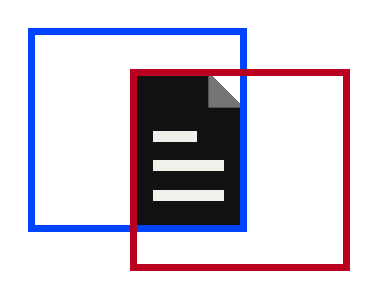
\begin{tikzpicture}[line join=miter, line cap=butt, miter limit=10]
  \ificon
    % square tile with a hard offset shadow, same language as the app's buttons
    \fill[edge] (-0.32,-1.18) rectangle (4.68,3.82);
    \fill[bgc] (-0.5,-1) rectangle (4.5,4);
    \draw[edge, line width=2.4pt] (-0.5,-1) rectangle (4.5,4);
  \fi

  % A ∩ B: the page, with a cut corner (fold)
  \fill[ink] (\bx,\ay) -- (\aX,\ay) -- (\aX,2.03) -- (2.25,\bY) -- (\bx,\bY) -- cycle;
  \fill[ink!55!bgc] (2.25,\bY) -- (2.25,2.03) -- (\aX,2.03) -- cycle;

  % text lines on the page
  \fill[bgc] (1.55,0.85) rectangle (2.45,0.99);
  \fill[bgc] (1.55,1.22) rectangle (2.45,1.36);
  \fill[bgc] (1.55,1.59) rectangle (2.10,1.73);

  % the two sets
  \draw[ca, line width=2.6pt] (\ax,\ay) rectangle (\aX,\aY);
  \draw[cb, line width=2.6pt] (\bx,\by) rectangle (\bX,\bY);

  \ifword
    % name: md in set-A colour, pdf in set-B colour, the 2 in ink
    \node[anchor=west, inner sep=0pt, font=\jb\bfseries\fontsize{64}{64}\selectfont]
      at (4.9,1.42) {\textcolor{ca}{md}\textcolor{ink}{2}\textcolor{cb}{pdf}};
  \fi
\end{tikzpicture}
\end{document}
